\section{Messung des Staudruckes}

Dieser Versuchsteil dient als Vorbereitung für die kommenden Versuche. Um den am besten geeigneten Ort für die weiteren Messungen heraus zu finden wird die Windgeschwindigkeit an verschiedenen Orten gemessen, um somit herauszufinden, wo diese am konstantesten ist.

\subsection{Messaufbau}

Für den Versuch werden drei verschiedene Abstände vom Gebläseende gewählt, bei denen jeweils im Mittelpunkt und für fünf unterschiedlichen Abstände dessen gemessen wird. Da das System invariant ist unter Drehungen um die Mittelpunktachse des Gebläses werden der Einfachheit halber die Abstände vom Mittelpunkt nach oben gewählt.

\subsection{Auswertung}

Wie man an den im Plot aufgetragenen Werten für die verschiedene Abstände zum Gebläse erkennen kann, ist die Luftgeschwindigkeit desto konstanter umso kleiner die Entfernung zum Ende des Gebläses ist und auch umso kleiner der Abstand zur Mittelpunktachse ist.
Deshalb wird für die kommenden Messungen ein Abstand von \SI{10}{\centi\metre} festgelegt und möglichst zentral vor dem Gebläse gemessen.

\begin{figure}[h!]
    \centering
    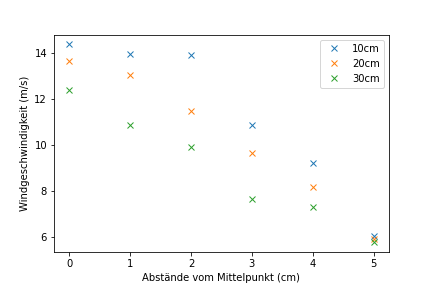
\includegraphics[scale=0.8]{Aeromechanik/Protokoll/fig/Aeromechanik Versuch 1.1.png}
    \caption{Windgeschwindigkeiten für drei verschiedene Abstände vom Gebläse}
    \label{fig:Aeromechanik Versuch 1.1}
\end{figure}

\section{Messung der Windgeschwindigkeit}

In diesem vorbereitenden Versuch geht es darum, die Abhängigkeit zwischen der Drehzahl des Gebläses und der Windgeschwindigkeit zu bestimmen. Um dies für die folgenden Versuche zu nutzen und somit Werte in Abhängigkeit von der Windgeschwindigkeit auszurechnen.

\subsection{Messaufbau}

\begin{figure}[h!]
    \centering
    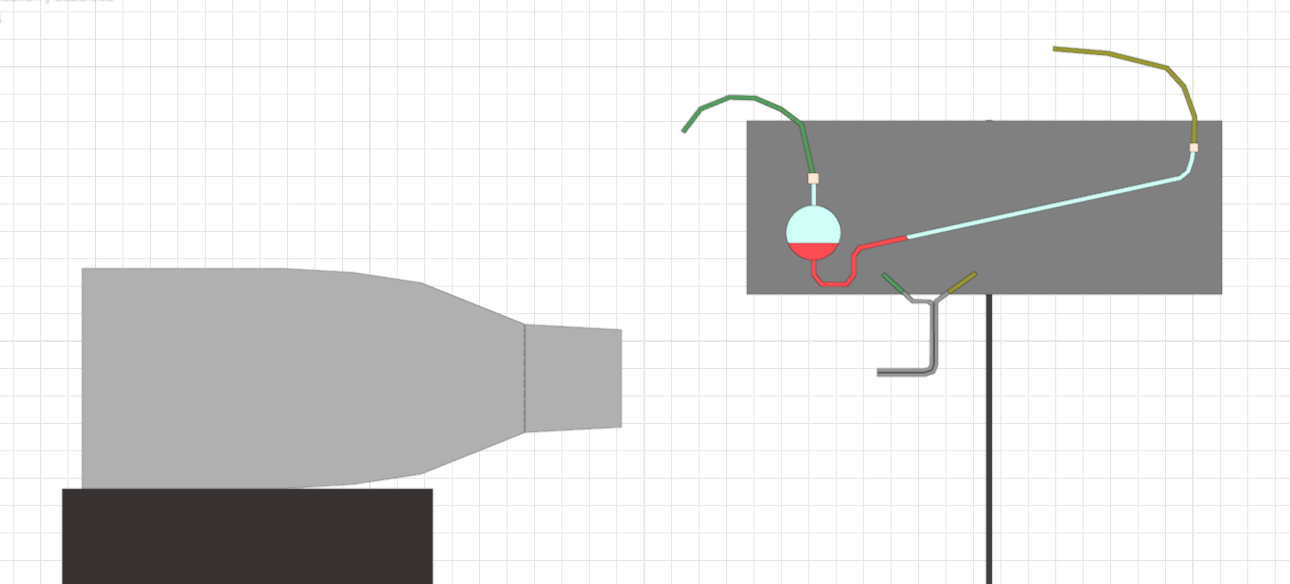
\includegraphics[scale=0.3]{Aeromechanik/Protokoll/fig/Kombi_Sonde.png}
    \caption{Versuchsaufbau mit Gebläse und kombininierter Sonde}
    \label{fig:Aeromechanik Versuch 1.2}
\end{figure}


Um den Versuch zu realisieren, wird der dynamische Druck mithilfe einer kombinierten Sonde gemessen. Wobei hierbei die Differenz zwischen statischem- und Gesamtdruck gemessen wird (vergleiche Demonstrationsversuche). Um nun aus den errechneten Wertepaaren aus dynamischen Druck und Drehzahl Werte für die Windgeschwindigkeit in Abhängigkeit von der Drehzahl aufzustellen, wird die Formel für den dynamischen Druck zu Rate gezogen: 

\begin{equation}
    p_{dyn} = \frac{\rho}{2} \cdot u^2
    \Rightarrow u = \sqrt{\frac{2p_{dyn}}{\rho}}
\end{equation}

Wobei die positive Wurzel gewählt wird um ein positives Ergebnis für die Geschwindigkeit zu erhalten, außerdem wird für die Dichte, die Dichte von Luft eingesetzt: $\rho = \SI{1.2}{\kg\per\cubic\m}$.

\begin{figure}[h!]
    \centering
    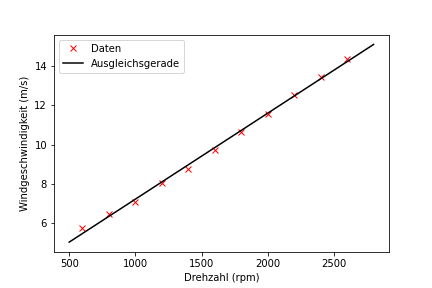
\includegraphics[scale=0.8]{Aeromechanik/Protokoll/fig/Aeromechanik Versuch 1.2.png}
    \caption{Windgeschwindigkeiten für verschiedene Drehzahlen}
    \label{fig:Aeromechanik Versuch 1.2}
\end{figure}